\documentclass[aspectratio=169]{beamer}

\usepackage[utf8]{inputenc}
\usepackage[english]{babel}
\usepackage{booktabs}
\usepackage{array}
\usepackage{listings}
\usepackage{tikz}
\usetikzlibrary{arrows.meta,positioning,shapes.geometric,calc,decorations.pathreplacing}

\graphicspath{{logo/}{../logo/}}

\definecolor{ForestGreen}{RGB}{22,100,70}
\definecolor{SoftGreen}{RGB}{229,244,235}
\definecolor{SoftBlue}{RGB}{226,239,255}
\definecolor{SoftOrange}{RGB}{255,241,220}
\definecolor{SoftPurple}{RGB}{239,231,255}

\newcolumntype{L}[1]{>{\raggedright\arraybackslash}p{#1}}

\mode<presentation>{
  \usetheme{Ilmenau}
  \usecolortheme{spruce}
  \usefonttheme{professionalfonts}
  \setbeamertemplate{navigation symbols}{}
  \setbeamertemplate{headline}{}
  \setbeamertemplate{caption}[numbered]
  \setbeamercolor{institute in head/foot}{fg=ForestGreen}
}

\lstdefinestyle{pseudo}{
  language={},
  basicstyle=\ttfamily\scriptsize,
  keywordstyle=\color{blue!75!black}\bfseries,
  morekeywords={FUNCTION,INPUT,OUTPUT,IF,THEN,ELSE,RETURN,FOR,TO,DO,WHILE,
    NONE,SWAP,LENGTH,APPEND,INSERT,EXTRACT,MINIMUM},
  numbers=none,
  showstringspaces=false,
  keepspaces=true,
  columns=fullflexible,
  breaklines=true,
  frame=single,
  rulecolor=\color{ForestGreen!60},
  backgroundcolor=\color{SoftBlue!35},
  tabsize=4
}

% Hide non-positive header line numbers; algorithm steps begin visibly at 1.
\newcommand{\pseudonumberstyle}{%
  \tiny\ifnum\value{lstnumber}>0\color{gray}\else\color{white}\fi}
\lstdefinestyle{pseudonumbered}{
  style=pseudo,
  numbers=left,
  firstnumber=-2,
  numberstyle=\pseudonumberstyle,
  numbersep=6pt,
  numberblanklines=false
}

\tikzset{
  cell/.style={draw=ForestGreen,fill=SoftGreen,thick,minimum width=0.82cm,
    minimum height=0.72cm,align=center},
  active/.style={draw=orange!75!black,fill=SoftOrange,very thick,
    minimum width=0.82cm,minimum height=0.72cm,align=center},
  found/.style={draw=purple!70!black,fill=SoftPurple,very thick,
    minimum width=0.82cm,minimum height=0.72cm,align=center},
  process/.style={draw=ForestGreen,rounded corners,fill=SoftGreen,thick,
    minimum height=0.9cm,text width=2.7cm,align=center},
  arrow/.style={-Latex,very thick,ForestGreen}
}

\title[TOKT11105 -- Lecture 4]{Data Structures and Algorithms in Python\\
Lecture 4: Sorting, Selection and Searching Algorithms}
\author{Faculty of Data Science and Artificial Intelligence}
\institute{National Economics University}
\date{}

\AtBeginSection[]{
  \begin{frame}[plain]
    \begin{center}
      \vfill
      {\color{ForestGreen}\large\bfseries SECTION \insertsectionnumber}
      \vspace{0.8em}
      {\color{ForestGreen}\rule{0.68\textwidth}{1.2pt}}
      \vspace{1.1em}
      {\usebeamerfont{section title}\color{ForestGreen}\LARGE\bfseries
        \parbox{0.86\textwidth}{\centering\insertsectionhead\par}}
      \vspace{1.1em}
      {\color{ForestGreen}\rule{0.68\textwidth}{1.2pt}}
      \vfill
    \end{center}
  \end{frame}
}

\begin{document}

\begin{frame}[plain]
  \setbeamercolor{block body example}{bg=ForestGreen,fg=white}
  \begin{center}
    \begin{beamercolorbox}[wd=\textwidth,sep=1pt,center,rounded=true,shadow=true]{block body example}
      \IfFileExists{logo_slide.png}{\includegraphics[width=0.27\textwidth]{logo_slide.png}}{{\vspace{0.7em}\Large\bfseries FDA -- NEU\vspace{0.7em}}}
    \end{beamercolorbox}
  \end{center}
  \vspace{-0.25em}
  \titlepage
\end{frame}

\logo{\IfFileExists{logo_fda.png}{\includegraphics[width=0.8cm]{logo_fda.png}}{}}
\setbeamercolor{footline upper}{bg=ForestGreen!22,fg=ForestGreen!85!black}
\setbeamercolor{footline lower}{bg=ForestGreen,fg=white}
\setbeamertemplate{footline}{%
  \leavevmode
  \hbox{%
    \begin{beamercolorbox}[wd=.50\paperwidth,ht=2.35ex,dp=.75ex,
      leftskip=1em]{footline upper}
      Faculty of Data Science and Artificial Intelligence
    \end{beamercolorbox}%
    \begin{beamercolorbox}[wd=.50\paperwidth,ht=2.35ex,dp=.75ex,
      rightskip=1em plus1fil]{footline upper}
      \hfill National Economics University
    \end{beamercolorbox}%
  }
  \hbox{%
    \begin{beamercolorbox}[wd=.72\paperwidth,ht=2.35ex,dp=.75ex,
      leftskip=1em]{footline lower}
      \insertshorttitle
    \end{beamercolorbox}%
    \begin{beamercolorbox}[wd=.28\paperwidth,ht=2.35ex,dp=.75ex,
      rightskip=1em plus1fil]{footline lower}
      \hfill Slide \insertframenumber/\inserttotalframenumber
    \end{beamercolorbox}%
  }
}

\begin{frame}{Lecture 4, Part 2: Table of Contents}
  \tableofcontents[hideallsubsections]
\end{frame}

\begin{frame}{Learning outcomes}
  By the end of this lecture, students should be able to:
  \begin{enumerate}
    \item Distinguish selection from complete sorting.
    \item Find extremes, order statistics, and top-$k$ values efficiently.
    \item Explain when sorting, quickselect, or a heap is appropriate.
    \item Implement linear, binary, and ternary search in pseudocode.
    \item Choose a search method based on data organization and workload.
  \end{enumerate}
\end{frame}

% =============================================================
\section{ Selection}
% =============================================================

\begin{frame}{Selection asks for part of the order}
  \begin{block}{Selection problem}
    Given $n$ values, find the record with rank $k$ without necessarily sorting
    every record.
  \end{block}
  \begin{columns}[T]
    \begin{column}{0.48\textwidth}
      \begin{exampleblock}{Examples}
        \begin{itemize}
          \item Minimum or maximum
          \item Median
          \item Third-smallest value
          \item Top ten scores
        \end{itemize}
      \end{exampleblock}
    \end{column}
    \begin{column}{0.48\textwidth}
      \begin{alertblock}{Key question}
        If only one rank is required, is the work of completely sorting the
        input necessary?
      \end{alertblock}
    \end{column}
  \end{columns}
\end{frame}

\begin{frame}{Rank and order statistics}
  \small
  \begin{block}{Sorted view of the running example}
    \[
      [7,3,5,2,6,4]\quad\longrightarrow\quad[2,3,4,5,6,7]
    \]
  \end{block}
  \begin{center}
    \begin{tabular}{ccc}
      \toprule
      \textbf{Request} & \textbf{Rank} & \textbf{Answer} \\
      \midrule
      Minimum & $1$ & $2$ \\
      Middle order statistics & $3,4$ & $4,5$ \\
      Fifth-smallest & $5$ & $6$ \\
      Maximum & $6$ & $7$ \\
      \bottomrule
    \end{tabular}
  \end{center}
  \begin{alertblock}{Convention}
    State whether ranks start at $1$ or $0$. In this lecture, ``$k$th smallest''
    uses ranks $1$ through $n$. For an even number of numerical values, the
    conventional median often averages the two middle order statistics.
  \end{alertblock}
\end{frame}

\begin{frame}[fragile]{Finding an extreme needs only one scan}
  \begin{columns}[T]
    \begin{column}{0.57\textwidth}
\begin{lstlisting}[style=pseudonumbered]
FUNCTION MINIMUM(A)
INPUT: non-empty array A
OUTPUT: smallest value in A
    best = A[0]
    FOR i = 1 TO LENGTH(A) - 1 DO
        IF A[i] < best THEN
            best = A[i]
    RETURN best
\end{lstlisting}
    \end{column}
    \begin{column}{0.39\textwidth}
      \begin{block}{Exact comparison count}
        Every value after the first is compared once:
        \[
          T(n)=n-1.
        \]
      \end{block}
      \begin{exampleblock}{Complexity}
        Time $\Theta(n)$; auxiliary space $\Theta(1)$. The maximum algorithm is
        identical except that $<$ is replaced by $>$.
      \end{exampleblock}
    \end{column}
  \end{columns}
\end{frame}

\begin{frame}{Strategies for the $k$th-smallest value}
  \small
  \begin{center}
    \begin{tabular}{L{0.24\textwidth}L{0.25\textwidth}L{0.35\textwidth}}
      \toprule
      \textbf{Strategy} & \textbf{Typical time} & \textbf{When useful} \\
      \midrule
      Sort, then index & $\Theta(n\log n)$ & Many later rank queries or sorted output needed \\
      Repeat minimum selection & $\Theta(kn)$ & Very small $k$, simple implementation \\
      Quickselect & Expected $\Theta(n)$ & One rank query on an in-memory array \\
      \bottomrule
    \end{tabular}
  \end{center}
  \begin{alertblock}{Algorithm design principle}
    Solve only the amount of ordering that the required output needs.
  \end{alertblock}
\end{frame}

\begin{frame}{Quickselect reuses quicksort's partition}
  \begin{block}{Core idea}
    Partition around a pivot. The pivot's final index tells us which side can
    contain the requested rank; discard the other side.
  \end{block}
  \begin{center}
    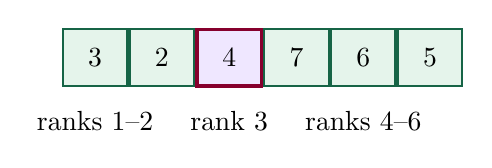
\begin{tikzpicture}[node distance=0pt]
      \node[cell] (a0) {3};
      \node[cell,right=of a0] (a1) {2};
      \node[found,right=of a1] (a2) {4};
      \node[cell,right=of a2] (a3) {7};
      \node[cell,right=of a3] (a4) {6};
      \node[cell,right=of a4] (a5) {5};
      \node[below=0.18cm of a0] {ranks 1--2};
      \node[below=0.18cm of a2] {rank 3};
      \node[below=0.18cm of a4] {ranks 4--6};
    \end{tikzpicture}
  \end{center}
  \begin{exampleblock}{Example}
    To find the fifth-smallest value, ignore the pivot and the entire left
    partition; continue only in the right partition.
  \end{exampleblock}
\end{frame}

\begin{frame}{Trace quickselect for the fifth-smallest value}
  \small
  \textbf{One possible execution:} the exact trace depends on pivot choices.
  \begin{center}
    \begin{tabular}{ccl}
      \toprule
      \textbf{Active range} & \textbf{Pivot rank} & \textbf{Decision} \\
      \midrule
      $[7,3,5,2,6,4]$ & $4$ becomes rank $3$ & Search ranks $4$--$6$ \\
      $[7,6,5]$ & $5$ becomes rank $4$ & Search ranks $5$--$6$ \\
      $[7,6]$ & $6$ becomes rank $5$ & Return $6$ \\
      \bottomrule
    \end{tabular}
  \end{center}
  \begin{alertblock}{What is avoided?}
    The elements with ranks below the pivot never need further processing.
  \end{alertblock}
  \begin{block}{State to track}
    The active bounds and the target index, not a fully sorted prefix.
  \end{block}
\end{frame}

\begin{frame}[fragile]{Quickselect pseudocode}
  \begin{columns}[T]
    \begin{column}{0.60\textwidth}
\begin{lstlisting}[style=pseudonumbered]
FUNCTION QUICKSELECT(A, k)
INPUT: array A and rank k, 1 <= k <= LENGTH(A)
OUTPUT: kth-smallest value
    target = k - 1
    low = 0; high = LENGTH(A) - 1
    WHILE low <= high DO
        p = PARTITION(A, low, high)
        IF p == target THEN
            RETURN A[p]
        ELSE IF target < p THEN
            high = p - 1
        ELSE
            low = p + 1
\end{lstlisting}
    \end{column}
    \begin{column}{0.36\textwidth}
      \begin{block}{Invariant}
        The target value is always inside $A[low..high]$.
      \end{block}
      \begin{alertblock}{Side effect}
        Quickselect rearranges the array but does not completely sort it.
      \end{alertblock}
    \end{column}
  \end{columns}
\end{frame}

\begin{frame}{Quickselect complexity}
  \small
  \begin{columns}[T]
    \begin{column}{0.48\textwidth}
      \begin{exampleblock}{Intuition with balanced partitions}
        \[
          n+\frac n2+\frac n4+\cdots < 2n
        \]
        Only one side is searched after each partition.
      \end{exampleblock}
    \end{column}
    \begin{column}{0.48\textwidth}
      \begin{alertblock}{Repeated poor pivots}
        \[
          n+(n-1)+(n-2)+\cdots
        \]
        Worst-case running time is $\Theta(n^2)$.
      \end{alertblock}
    \end{column}
  \end{columns}
  \begin{block}{Practical protection}
    With randomized pivots, Quickselect has expected $\Theta(n)$ time and
    consistently unbalanced partitions become unlikely.
  \end{block}
\end{frame}

\begin{frame}{Median of medians: choosing a reliable pivot}
  \small
  \begin{block}{Idea}
    Instead of choosing an arbitrary quickselect pivot, divide the input into
    groups of five, find each group median, then select the median of those
    medians as the pivot.
  \end{block}
  \begin{center}
    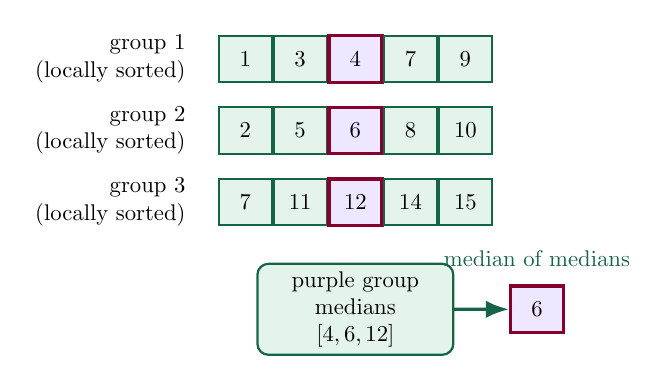
\begin{tikzpicture}[node distance=0pt,scale=0.82,transform shape]
      \node[cell] (g10) {1};
      \node[cell,right=of g10] (g11) {3};
      \node[found,right=of g11] (g12) {4};
      \node[cell,right=of g12] (g13) {7};
      \node[cell,right=of g13] (g14) {9};
      \node[left=0.38cm of g10,align=right] {group 1\\(locally sorted)};

      \node[cell,below=0.36cm of g10] (g20) {2};
      \node[cell,right=of g20] (g21) {5};
      \node[found,right=of g21] (g22) {6};
      \node[cell,right=of g22] (g23) {8};
      \node[cell,right=of g23] (g24) {10};
      \node[left=0.38cm of g20,align=right] {group 2\\(locally sorted)};

      \node[cell,below=0.36cm of g20] (g30) {7};
      \node[cell,right=of g30] (g31) {11};
      \node[found,right=of g31] (g32) {12};
      \node[cell,right=of g32] (g33) {14};
      \node[cell,right=of g33] (g34) {15};
      \node[left=0.38cm of g30,align=right] {group 3\\(locally sorted)};

      \node[process,text width=2.8cm,below=0.56cm of g32] (medians)
        {purple group medians\\$[4,6,12]$};
      \node[found,right=0.85cm of medians] (pivot) {6};
      \node[above=0.16cm of pivot,ForestGreen] {median of medians};
      \draw[arrow] (medians) -- (pivot);
    \end{tikzpicture}
  \end{center}
  \centering\footnotesize
  \textbf{Important:} for a large list of group medians, find their median
  recursively. The resulting pivot need not be the original array's true median.
\end{frame}

\begin{frame}{Advanced note: median of medians and linear worst case}
  \footnotesize
  \begin{columns}[T]
    \begin{column}{0.48\textwidth}
      \begin{block}{A guaranteed useful pivot}
        There are about $n/5$ groups. At least half of their medians are at
        least the chosen pivot $p$, and each such group contains three values
        at least $p$. The same argument holds on the smaller side.
        \[
          \text{At least }\frac{3n}{10}-O(1)
        \]
        values can be discarded from either side; the remaining subproblem has
        size at most $7n/10+O(1)$.
      \end{block}
    \end{column}
    \begin{column}{0.48\textwidth}
      \begin{alertblock}{Recurrence and result}
        \[
          T(n)\le T(\lceil n/5\rceil)
          +T(7n/10+O(1))+cn.
        \]
        The recursive fractions satisfy
        \[
          \frac15+\frac7{10}=\frac9{10}<1,
        \]
        so the recurrence is $O(n)$. Since selection must inspect the input,
        it is also $\Omega(n)$; therefore the deterministic worst-case time is
        \[
          \Theta(n).
        \]
      \end{alertblock}
    \end{column}
  \end{columns}
\end{frame}

\begin{frame}{Finding top-$k$ values}
  \small
  \begin{block}{Problem}
    Return the $k$ largest or $k$ smallest values without necessarily sorting
    all $n$ input values.
  \end{block}
  \begin{center}
    \begin{tabular}{L{0.25\textwidth}L{0.22\textwidth}L{0.34\textwidth}}
      \toprule
      \textbf{Method} & \textbf{Typical time} & \textbf{When useful} \\
      \midrule
      Sort all values & $\Theta(n\log n)$ & Need complete sorted output \\
      Quickselect, then scan & Expected $\Theta(n)$ & Need only the top-$k$ set \\
      Heap of size $k$ & $O(n\log k)$ & $k\ll n$ or data arrives as a stream \\
      \bottomrule
    \end{tabular}
  \end{center}
  \begin{alertblock}{Key idea}
    Top-$k$ is between selection and sorting: more than one rank is needed, but
    a complete total order may still be unnecessary.
  \end{alertblock}
\end{frame}

\begin{frame}{Self-check: selection}
  \small
  \begin{enumerate}
    \item In $[8,2,9,1,5,7]$, what is the fourth-smallest value?
    \item Why does finding the minimum not require sorting?
    \item When is sorting better than Quickselect for rank queries?
    \item For $k=10$ and very large $n$, why can a heap of size $k$ be useful?
    \item Does Quickselect return a fully sorted array? Explain briefly.
  \end{enumerate}
  \begin{block}{Discussion rule}
    Give the answer, then justify it using the required amount of ordering.
  \end{block}
\end{frame}

\begin{frame}{Activity: choose a selection method}
  \begin{columns}[T]
    \begin{column}{0.51\textwidth}
      \begin{block}{Scenarios}
        \begin{enumerate}
          \item Find one median in an unsorted array.
          \item Report the ten largest values after all data is collected.
          \item Answer thousands of rank queries on fixed data.
          \item Find only the minimum value.
        \end{enumerate}
      \end{block}
    \end{column}
    \begin{column}{0.45\textwidth}
      \begin{alertblock}{Student task}
        Choose among scanning, sorting, quickselect, and a heap. Explain the
        required time, memory, and whether input modification is acceptable.
      \end{alertblock}
    \end{column}
  \end{columns}
\end{frame}

% =============================================================
\section{ Searching}
% =============================================================

\begin{frame}{The searching problem}
  \begin{block}{Input and output}
    Given a collection and a target key, return a matching position or record;
    return \texttt{NONE} when no match exists.
  \end{block}
  \begin{columns}[T]
    \begin{column}{0.48\textwidth}
      \begin{exampleblock}{Questions to specify}
        \begin{itemize}
          \item Is the collection ordered?
          \item Are duplicate keys allowed?
          \item Return first, last, any, or all matches?
        \end{itemize}
      \end{exampleblock}
    \end{column}
    \begin{column}{0.48\textwidth}
      \begin{alertblock}{Cost model}
        Count key comparisons and any preprocessing needed to organize the data.
      \end{alertblock}
    \end{column}
  \end{columns}
\end{frame}

\begin{frame}{Linear search: inspect values from left to right}
  \begin{center}
    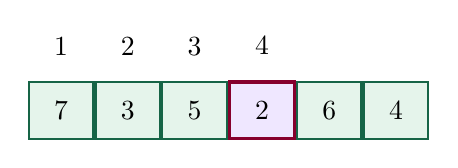
\begin{tikzpicture}[node distance=0pt]
      \node[cell] (a0) {7};
      \node[cell,right=of a0] (a1) {3};
      \node[cell,right=of a1] (a2) {5};
      \node[found,right=of a2] (a3) {2};
      \node[cell,right=of a3] (a4) {6};
      \node[cell,right=of a4] (a5) {4};
      \node[above=0.2cm of a0] {1};
      \node[above=0.2cm of a1] {2};
      \node[above=0.2cm of a2] {3};
      \node[above=0.2cm of a3] {4};
    \end{tikzpicture}
  \end{center}
  \begin{block}{Target $2$}
    The first match occurs after four comparisons. Values after the match are
    not inspected.
  \end{block}
  \begin{alertblock}{No ordering assumption}
    Linear search works on arbitrary sequences and linked structures.
  \end{alertblock}
\end{frame}

\begin{frame}[fragile]{Linear-search pseudocode and cases}
  \begin{columns}[T]
    \begin{column}{0.56\textwidth}
\begin{lstlisting}[style=pseudonumbered]
FUNCTION LINEAR_SEARCH(A, target)
INPUT: array A and a target value
OUTPUT: an index of target, or NONE
    FOR i = 0 TO LENGTH(A) - 1 DO
        IF A[i] == target THEN
            RETURN i
    RETURN NONE
\end{lstlisting}
    \end{column}
    \begin{column}{0.40\textwidth}
      \begin{block}{Comparisons}
        Best: $1$\\
        Worst: $n$\\
        Average successful search: about $(n+1)/2$ when all positions are equally likely
      \end{block}
      \begin{exampleblock}{Complexity}
        Best $\Theta(1)$; average and worst $\Theta(n)$.
      \end{exampleblock}
    \end{column}
  \end{columns}
\end{frame}


\begin{frame}{Can ordering help us search faster?}
  \small
  \begin{columns}[T]
    \begin{column}{0.48\textwidth}
      \begin{alertblock}{Unsorted data}
        \[
          [7,3,5,2,6,4]
        \]
        No position rule tells us where the target might be. In the worst case,
        every value may need inspection.
      \end{alertblock}
    \end{column}
    \begin{column}{0.48\textwidth}
      \begin{exampleblock}{Sorted data}
        \[
          [2,3,4,5,6,7]
        \]
        Comparing with the middle value tells us which half cannot contain the
        target.
      \end{exampleblock}
    \end{column}
  \end{columns}
  \begin{block}{Main message}
    Fast search usually comes from extra structure in the data representation.
  \end{block}
\end{frame}

\begin{frame}{Binary search requires sorted data}
  \begin{block}{Precondition}
    The searched keys must already be ordered. Binary search compares the target
    with the middle value and discards half of the remaining range.
  \end{block}
  \begin{center}
    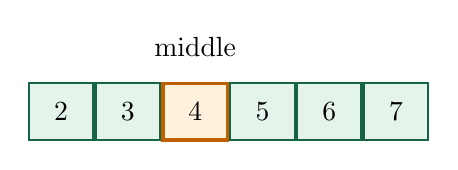
\begin{tikzpicture}[node distance=0pt]
      \node[cell] (a0) {2};
      \node[cell,right=of a0] (a1) {3};
      \node[active,right=of a1] (a2) {4};
      \node[cell,right=of a2] (a3) {5};
      \node[cell,right=of a3] (a4) {6};
      \node[cell,right=of a4] (a5) {7};
      \node[above=0.2cm of a2] {middle};
    \end{tikzpicture}
  \end{center}
  \begin{alertblock}{Target $6$}
    Because $6>4$, indices to the left of and including the middle cannot
    contain the target.
  \end{alertblock}
\end{frame}

\begin{frame}{Trace binary search for target $6$}
  \small
  \begin{center}
    \begin{tabular}{cccccl}
      \toprule
      \textbf{Step} & \textbf{low} & \textbf{high} & \textbf{mid} &
      \textbf{$A[mid]$} & \textbf{Action} \\
      \midrule
      1 & $0$ & $5$ & $2$ & $4$ & discard indices $0..2$ \\
      2 & $3$ & $5$ & $4$ & $6$ & return index $4$ \\
      \bottomrule
    \end{tabular}
  \end{center}
  \begin{block}{Search interval invariant}
    If the target exists, at the start of every iteration it lies somewhere in
    the inclusive interval $[low,high]$.
  \end{block}
  \begin{exampleblock}{Progress}
    Each unsuccessful comparison strictly reduces the interval size.
  \end{exampleblock}
\end{frame}

\begin{frame}[fragile]{Iterative binary-search pseudocode}
  \begin{columns}[T]
    \begin{column}{0.58\textwidth}
\begin{lstlisting}[style=pseudonumbered]
FUNCTION BINARY_SEARCH(A, target)
INPUT: sorted array A
OUTPUT: an index of target, or NONE
    low = 0
    high = LENGTH(A) - 1
    WHILE low <= high DO
        mid = low + (high - low) DIV 2
        IF A[mid] == target THEN
            RETURN mid
        ELSE IF A[mid] < target THEN
            low = mid + 1
        ELSE
            high = mid - 1
    RETURN NONE
\end{lstlisting}
    \end{column}
    \begin{column}{0.38\textwidth}
      \begin{block}{Complexity}
        After $t$ steps the range has size at most $n/2^t$. Therefore the worst
        case is $\Theta(\log n)$.
      \end{block}
      \begin{alertblock}{Boundary condition}
        Use \texttt{low <= high}; an interval with one element still needs to be
        checked.
      \end{alertblock}
    \end{column}
  \end{columns}
\end{frame}

\begin{frame}{Why binary search is correct}
  \small
  \begin{enumerate}
    \item Initially, every valid index is inside $[low,high]$.
    \item If $A[mid]<target$, sorted order proves indices $low..mid$ cannot
      contain the target.
    \item If $A[mid]>target$, sorted order proves indices $mid..high$ cannot
      contain the target.
    \item The interval shrinks after every unsuccessful comparison.
    \item A match is returned, or the empty interval proves absence.
  \end{enumerate}
  \begin{alertblock}{Important distinction}
    Binary search is fast only after data is sorted. For one search, sorting an
    unsorted array first may cost more than a linear scan.
  \end{alertblock}
\end{frame}

\begin{frame}[fragile]{Variant: find the first occurrence}
  \begin{columns}[T]
    \begin{column}{0.59\textwidth}
\begin{lstlisting}[style=pseudonumbered]
FUNCTION FIRST_OCCURRENCE(A, target)
INPUT: sorted array A and a target value
OUTPUT: first index of target, or NONE
    low = 0; high = LENGTH(A) - 1
    answer = NONE
    WHILE low <= high DO
        mid = low + (high - low) DIV 2
        IF A[mid] >= target THEN
            IF A[mid] == target THEN answer = mid
            high = mid - 1
        ELSE
            low = mid + 1
    RETURN answer
\end{lstlisting}
    \end{column}
    \begin{column}{0.37\textwidth}
      \begin{block}{Why continue after a match?}
        A matching value may also occur at a smaller index, so remember the
        match and search left.
      \end{block}
      \begin{exampleblock}{Uses}
        Counting duplicates, locating ranges, and implementing lower-bound
        queries.
      \end{exampleblock}
    \end{column}
  \end{columns}
\end{frame}

\begin{frame}[fragile]{Searching with Python tools}
  \begin{columns}[T]
    \begin{column}{0.49\textwidth}
      \begin{block}{Sequence search}
\begin{lstlisting}[language=Python,basicstyle=\ttfamily\tiny]
target in values
values.index(target)
\end{lstlisting}
        These operations use a linear scan for a list.
      \end{block}
      \begin{exampleblock}{Ordered search}
\begin{lstlisting}[language=Python,basicstyle=\ttfamily\tiny]
from bisect import bisect_left
i = bisect_left(values, target)
found = i < len(values) and values[i] == target
\end{lstlisting}
      \end{exampleblock}
    \end{column}
    \begin{column}{0.49\textwidth}
      \begin{alertblock}{Set and dictionary lookup}
\begin{lstlisting}[language=Python,basicstyle=\ttfamily\tiny]
student_id in id_set
record = records_by_id.get(student_id)
\end{lstlisting}
        Hash-based lookup is expected $O(1)$, but requires extra storage and
        does not provide sorted-order queries.
      \end{alertblock}
    \end{column}
  \end{columns}
\end{frame}

\begin{frame}{Do not choose the algorithm alone}
  \scriptsize
  \begin{center}
    \begin{tabular}{L{0.19\textwidth}L{0.22\textwidth}L{0.19\textwidth}L{0.24\textwidth}}
      \toprule
      \textbf{Representation} & \textbf{Typical lookup} & \textbf{Update cost} & \textbf{Best fit} \\
      \midrule
      Unsorted list & Linear, $\Theta(n)$ & Append often $O(1)$ & Few searches, frequent simple inserts \\
      Sorted array/list & Binary, $\Theta(\log n)$ & Insert/delete $\Theta(n)$ & Many range or ordered queries \\
      Hash set/dict & Expected $O(1)$ & Expected $O(1)$ & Exact-key membership or retrieval \\
      Balanced search tree & $O(\log n)$ & $O(\log n)$ & Dynamic ordered data and range queries \\
      \bottomrule
    \end{tabular}
  \end{center}
  \begin{alertblock}{Whole-workload thinking}
    The best search algorithm depends on how the data was organized and how
    often searches and updates occur.
  \end{alertblock}
\end{frame}

\begin{frame}{Common binary-search mistakes}
  \begin{columns}[T]
    \begin{column}{0.48\textwidth}
      \begin{alertblock}{Frequent errors}
        \begin{itemize}
          \item Applying it to unsorted data
          \item Mixing inclusive and exclusive bounds
          \item Updating to \texttt{mid} instead of \texttt{mid +/- 1}
          \item Ignoring duplicate-key requirements
          \item Returning insertion position as a confirmed match
        \end{itemize}
      \end{alertblock}
    \end{column}
    \begin{column}{0.48\textwidth}
      \begin{exampleblock}{Testing checklist}
        Test an empty array, one element, target at each end, absent target,
        duplicates, and an even-length interval.
      \end{exampleblock}
      \begin{block}{Debugging tool}
        Trace \texttt{low}, \texttt{mid}, and \texttt{high} after every step.
      \end{block}
    \end{column}
  \end{columns}
\end{frame}


\begin{frame}{Self-check: searching}
  \small
  \begin{enumerate}
    \item Why is binary search invalid on an unsorted list?
    \item In binary search, why should an inclusive interval use \texttt{low <= high}?
    \item What should change if duplicate keys are allowed and the first match is required?
    \item Which structure is better for exact membership: list, sorted list, or hash set?
    \item Which structure is better for range queries: hash table or sorted structure?
  \end{enumerate}
  \begin{block}{Discussion rule}
    State the representation first, then state the search cost.
  \end{block}
\end{frame}

\begin{frame}{Integrated activity: product catalogue}
  \begin{block}{Situation}
    A catalogue receives 50 updates per day and serves 100,000 exact product-ID
    searches plus 2,000 price-range searches per day.
  \end{block}
  \begin{alertblock}{Student task}
    \begin{enumerate}
      \item Choose representations for exact-ID and price-range queries.
      \item Explain whether one structure is enough.
      \item State the expected lookup and update costs.
      \item Explain how sorting by price can report the ten most expensive products.
    \end{enumerate}
  \end{alertblock}
  \begin{exampleblock}{Design insight}
    Real systems often maintain more than one index because no single data
    organization is optimal for every query.
  \end{exampleblock}
\end{frame}

\begin{frame}{Optional: ternary search on a unimodal function}
  \scriptsize
  \begin{block}{Core idea}
    Ternary search can locate the optimum of a \textbf{unimodal function}:
    values increase then decrease, or decrease then increase, with one optimum.
  \end{block}
  \begin{columns}[T]
    \begin{column}{0.58\textwidth}
      \begin{exampleblock}{Single-peak shape}
      \begin{center}
      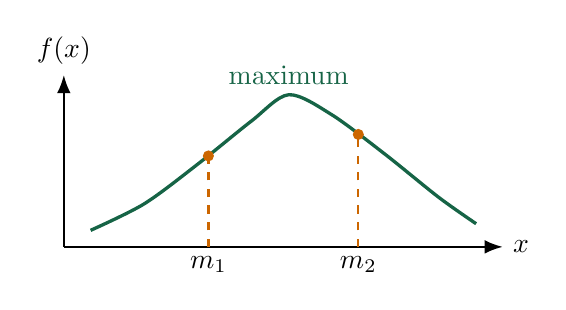
\begin{tikzpicture}[x=0.68cm,y=0.42cm]
        \draw[-Latex,thick] (0,0) -- (8.2,0) node[right] {$x$};
        \draw[-Latex,thick] (0,0) -- (0,5.2) node[above] {$f(x)$};
        \draw[ForestGreen,very thick,smooth]
          plot coordinates {(0.5,0.5) (1.5,1.3) (2.5,2.5) (3.5,3.8)
            (4.2,4.6) (5.0,4.0) (6.0,2.8) (7.0,1.5) (7.7,0.7)};
        \draw[dashed,orange!80!black,thick] (2.7,0) -- (2.7,2.75);
        \draw[dashed,orange!80!black,thick] (5.5,0) -- (5.5,3.4);
        \fill[orange!80!black] (2.7,2.75) circle (2pt);
        \fill[orange!80!black] (5.5,3.4) circle (2pt);
        \node[below] at (2.7,0) {$m_1$};
        \node[below] at (5.5,0) {$m_2$};
        \node[ForestGreen,above] at (4.2,4.6) {maximum};
      \end{tikzpicture}
      \end{center}
      \end{exampleblock}
    \end{column}
    \begin{column}{0.38\textwidth}
      \begin{exampleblock}{Example}
        Suppose $f(x)$ is profit at price $x$: profit rises, reaches one peak,
        then falls. Search for the price that maximizes profit.
      \end{exampleblock}
      \begin{alertblock}{One step for a maximum}
        If $f(m_1)<f(m_2)$, the maximum cannot lie to the left of $m_1$;
        discard that third. Otherwise, discard the part right of $m_2$.
      \end{alertblock}
    \end{column}
  \end{columns}
  \begin{block}{Stopping and complexity}
    Discrete interval: $\Theta(\log n)$ iterations. Continuous interval: stop
    when its width is within the required precision.
  \end{block}
\end{frame}


\begin{frame}[fragile]{Ternary-search pseudocode}
  \small
  \begin{columns}[T]
    \begin{column}{0.58\textwidth}
\begin{lstlisting}[style=pseudonumbered]
FUNCTION TERNARY_SEARCH_MAX(f, left, right, eps)
INPUT: unimodal function f on [left, right]
OUTPUT: approximate maximizer of f
    WHILE right - left > eps DO
        m1 = left + (right - left) / 3
        m2 = right - (right - left) / 3
        IF f(m1) < f(m2) THEN
            left = m1
        ELSE
            right = m2
    RETURN (left + right) / 2
\end{lstlisting}
    \end{column}
    \begin{column}{0.38\textwidth}
      \begin{block}{For a maximum}
        If $f(m_1)<f(m_2)$, the peak cannot be in the left third. Otherwise,
        discard the right third.
      \end{block}
      \begin{alertblock}{Precondition}
        Ternary search is valid only when the function or sequence is unimodal.
      \end{alertblock}
    \end{column}
  \end{columns}
\end{frame}

\begin{frame}[fragile]{Discrete ternary-search pseudocode}
  \small
\begin{lstlisting}[style=pseudonumbered]
FUNCTION TERNARY_SEARCH_MAX_ARRAY(A)
INPUT: unimodal array A
OUTPUT: index of a maximum value
    low = 0; high = LENGTH(A) - 1
    WHILE high - low > 3 DO
        m1 = low + (high - low) DIV 3
        m2 = high - (high - low) DIV 3
        IF A[m1] < A[m2] THEN
            low = m1 + 1
        ELSE
            high = m2 - 1
    best = low
    FOR i = low + 1 TO high DO
        IF A[i] > A[best] THEN best = i
    RETURN best
\end{lstlisting}
\end{frame}

\begin{frame}{Self-check: ternary search}
  \small
  \begin{enumerate}
    \item What property must the input satisfy before ternary search is valid?
    \item For maximizing profit by price, why might binary search not apply directly?
    \item In the maximum version, what can be discarded when $f(m_1)<f(m_2)$?
    \item Why does the discrete version scan the final small interval directly?
  \end{enumerate}
\end{frame}

\begin{frame}{Key takeaways}
  \small
  \begin{block}{Selection}
    Do not sort more than the output requires. Quickselect can find one order
    statistic in expected $\Theta(n)$ time; top-$k$ can often avoid full sorting.
  \end{block}
  \begin{block}{Searching}
    Without useful organization, search may require $\Theta(n)$ comparisons.
    Sorted order enables binary search in $\Theta(\log n)$.
  \end{block}
  \begin{alertblock}{Data-structure thinking}
    Search complexity cannot be separated from data organization, update cost,
    and query workload.
  \end{alertblock}
\end{frame}

\begin{frame}{After-class practice}
  \small
  \begin{enumerate}
    \item Trace quickselect for the third-smallest value of $[9,1,7,3,8,2,6]$.
    \item Design an algorithm that returns both minimum and maximum.
    \item Find the five largest values in a list without fully sorting it.
    \item Trace binary search for present and absent targets in an even-length array.
    \item Modify binary search to find the last occurrence of a duplicated key.
    \item Compare a list, sorted list, dictionary, and set for a student-ID system.
  \end{enumerate}
\end{frame}

\begin{frame}{Short programming exercises}
  \small
  \begin{enumerate}
    \item Write Python code for \texttt{minimum(values)} without using \texttt{min}.
    \item Write \texttt{linear\_search(values, target)} and count comparisons.
    \item Write \texttt{binary\_search(sorted\_values, target)} and print
      \texttt{low}, \texttt{mid}, and \texttt{high} at each step.
    \item Use \texttt{bisect\_left} to test whether a target occurs in a sorted list.
    \item Implement ternary search for a simple unimodal function, for example
      $f(x)=-(x-3)^2+10$.
  \end{enumerate}
\end{frame}

\end{document}